% Snippet para integrar os prints no Overleaf.
% No preambulo do artigo, adicione:
% \usepackage{graphicx}
% \usepackage{float}
%
% Envie a pasta screenshots para o Overleaf mantendo os mesmos nomes dos arquivos.

\section{Registros Visuais do Sistema}

\begin{figure}[H]
    \centering
    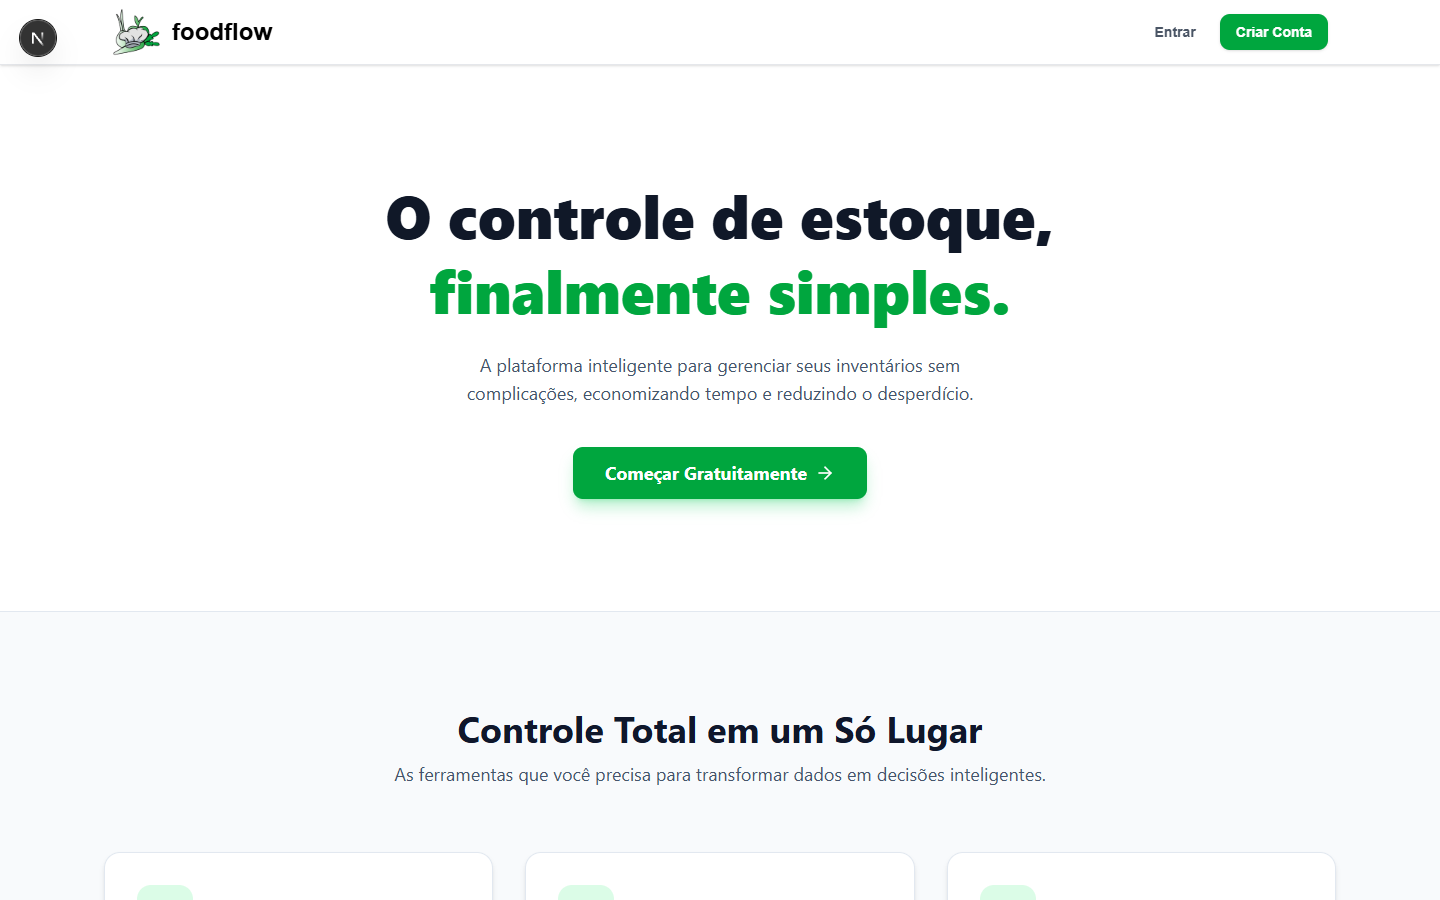
\includegraphics[width=\textwidth]{screenshots/01_home.png}
    \caption{Pagina inicial do FoodFlow.}
\end{figure}

\begin{figure}[H]
    \centering
    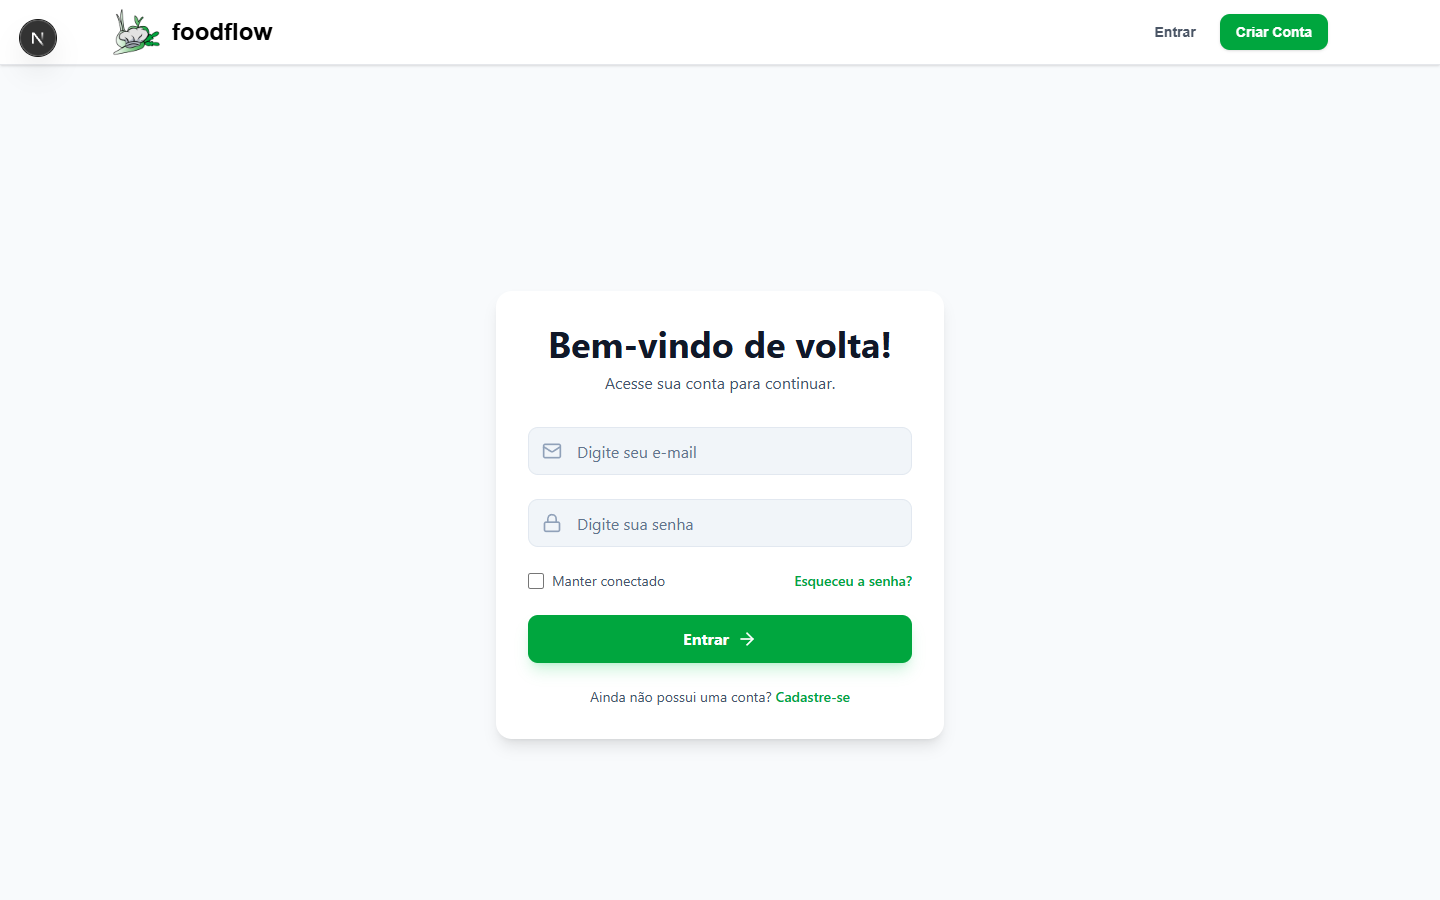
\includegraphics[width=\textwidth]{screenshots/02_login.png}
    \caption{Tela de login.}
\end{figure}

\begin{figure}[H]
    \centering
    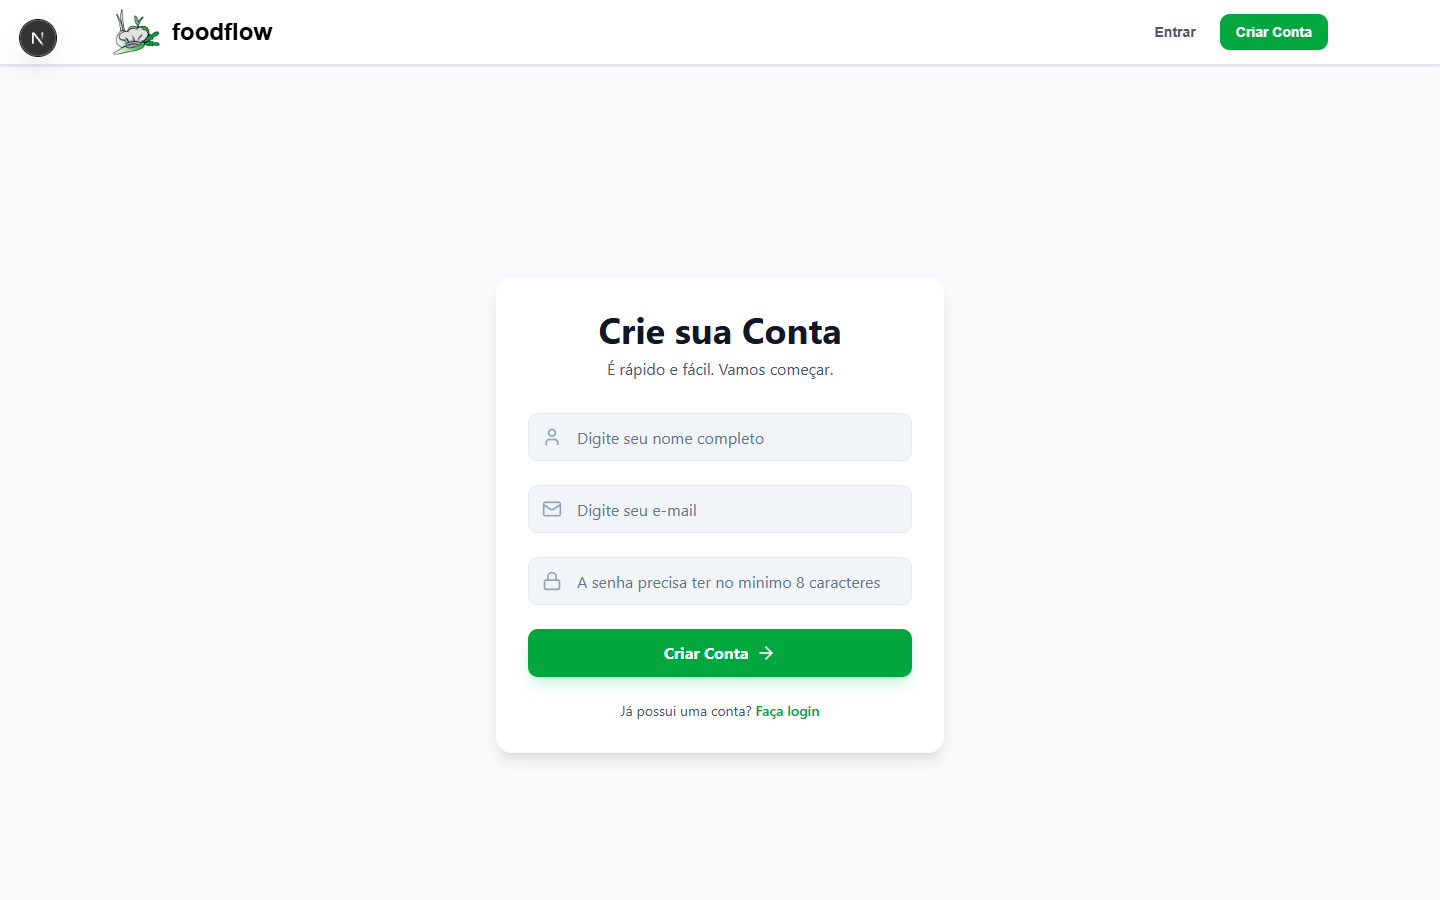
\includegraphics[width=\textwidth]{screenshots/03_cadastro.png}
    \caption{Tela de cadastro de usuario.}
\end{figure}

\begin{figure}[H]
    \centering
    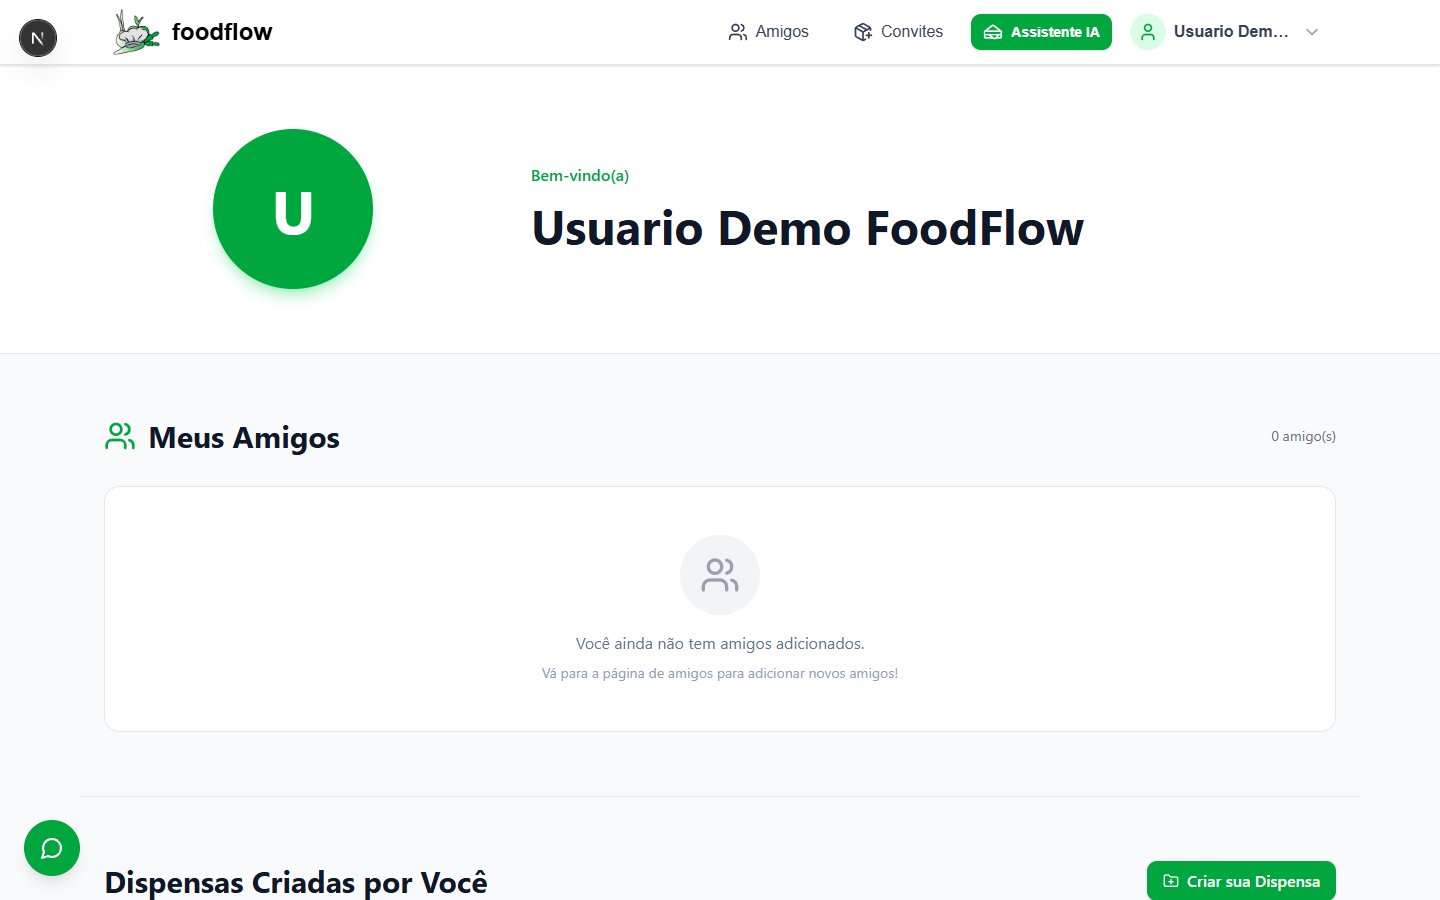
\includegraphics[width=\textwidth]{screenshots/04_perfil_dispensas_amigos.png}
    \caption{Perfil com amigos e dispensas vinculadas ao usuario.}
\end{figure}

\begin{figure}[H]
    \centering
    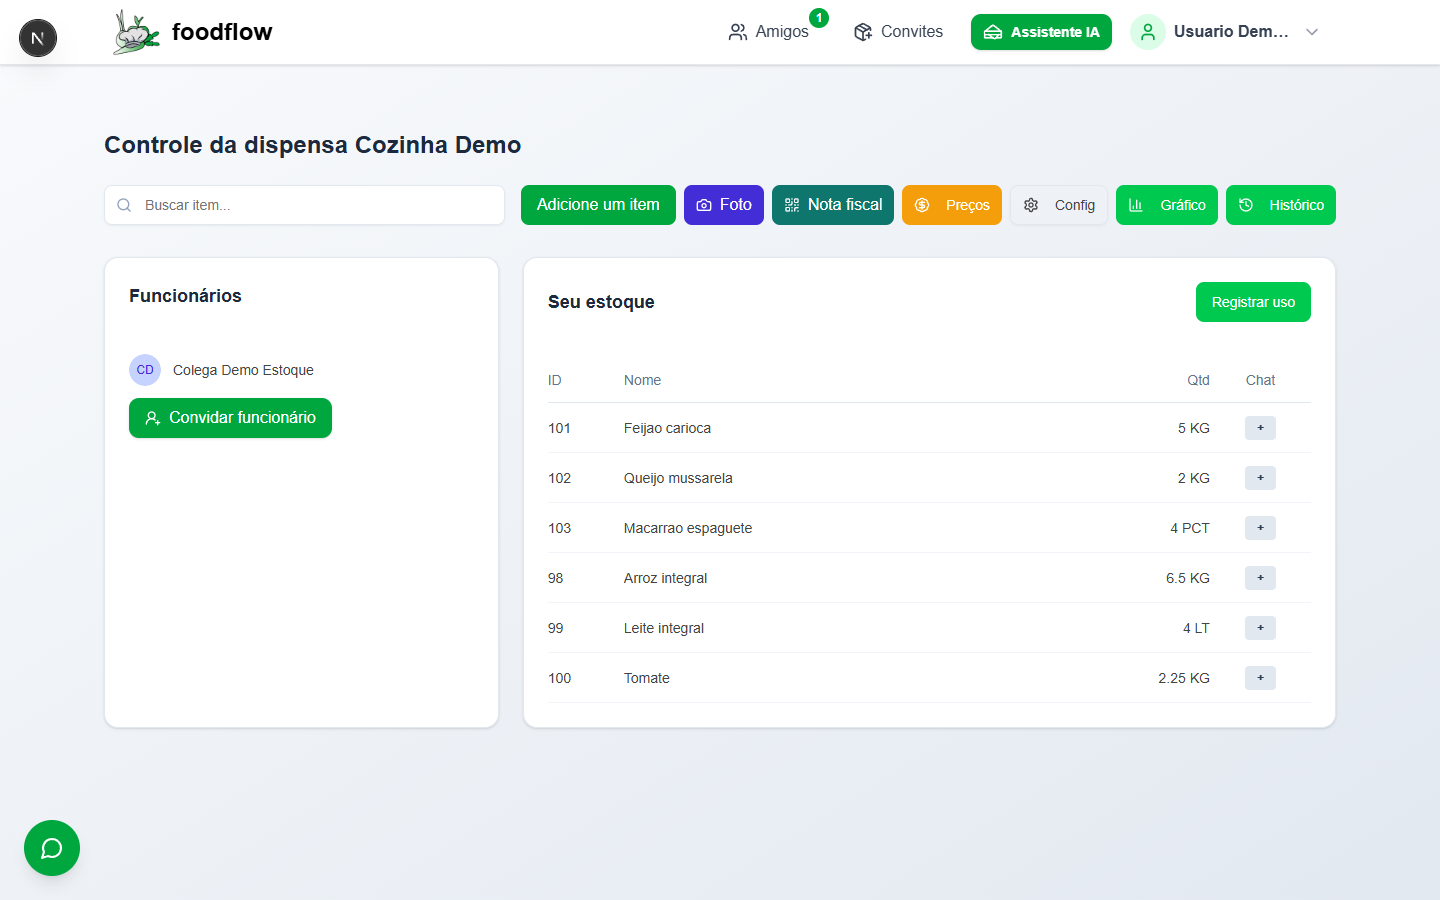
\includegraphics[width=\textwidth]{screenshots/05_dispensa_estoque.png}
    \caption{Tela principal da dispensa com estoque cadastrado.}
\end{figure}

\begin{figure}[H]
    \centering
    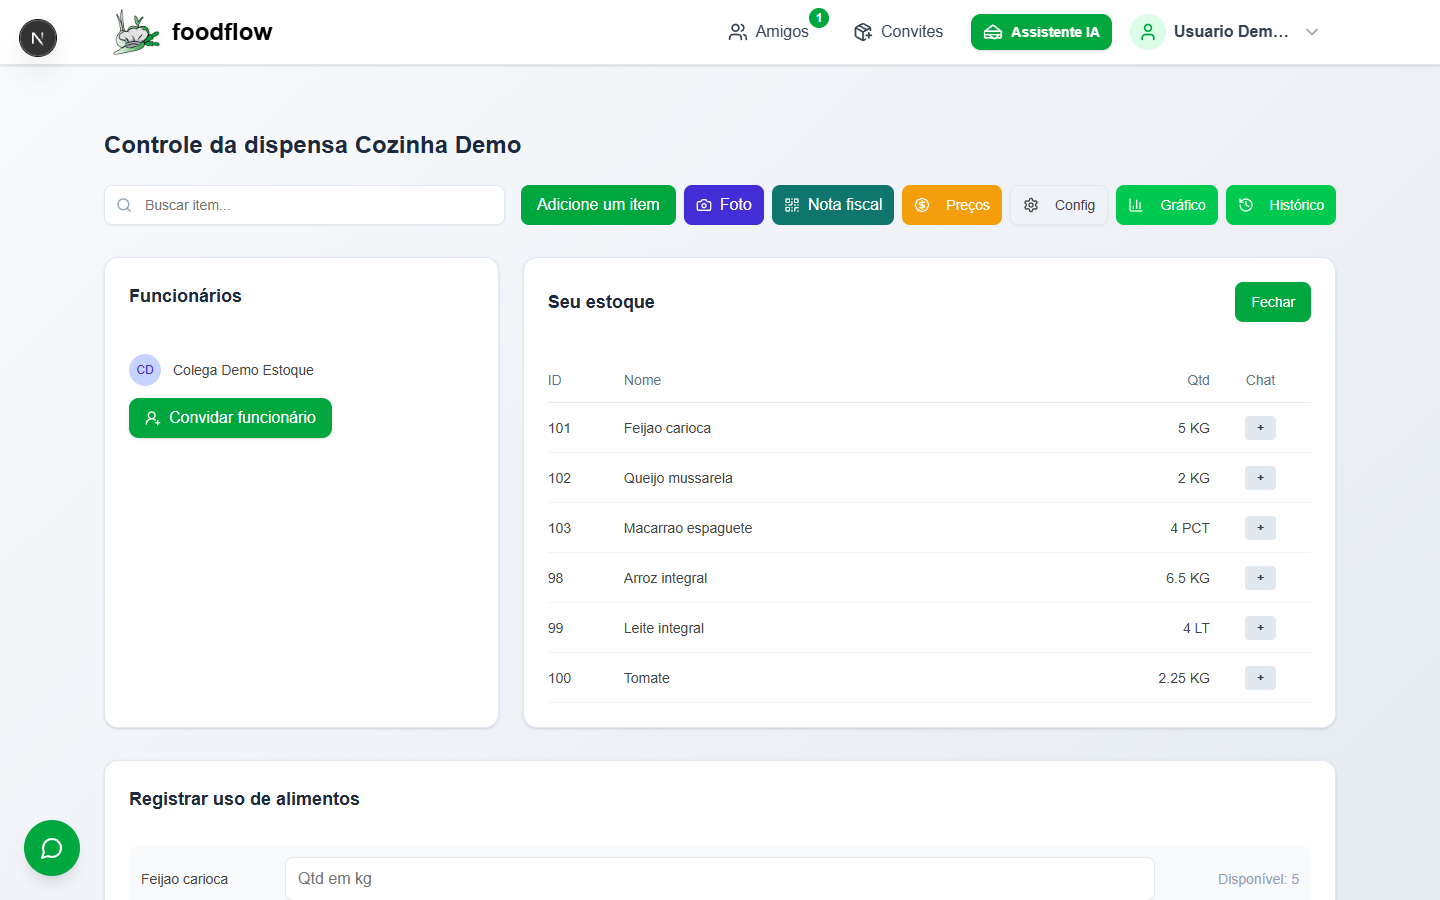
\includegraphics[width=\textwidth]{screenshots/06_dispensa_registrar_uso.png}
    \caption{Formulario de registro de uso de alimentos.}
\end{figure}

\begin{figure}[H]
    \centering
    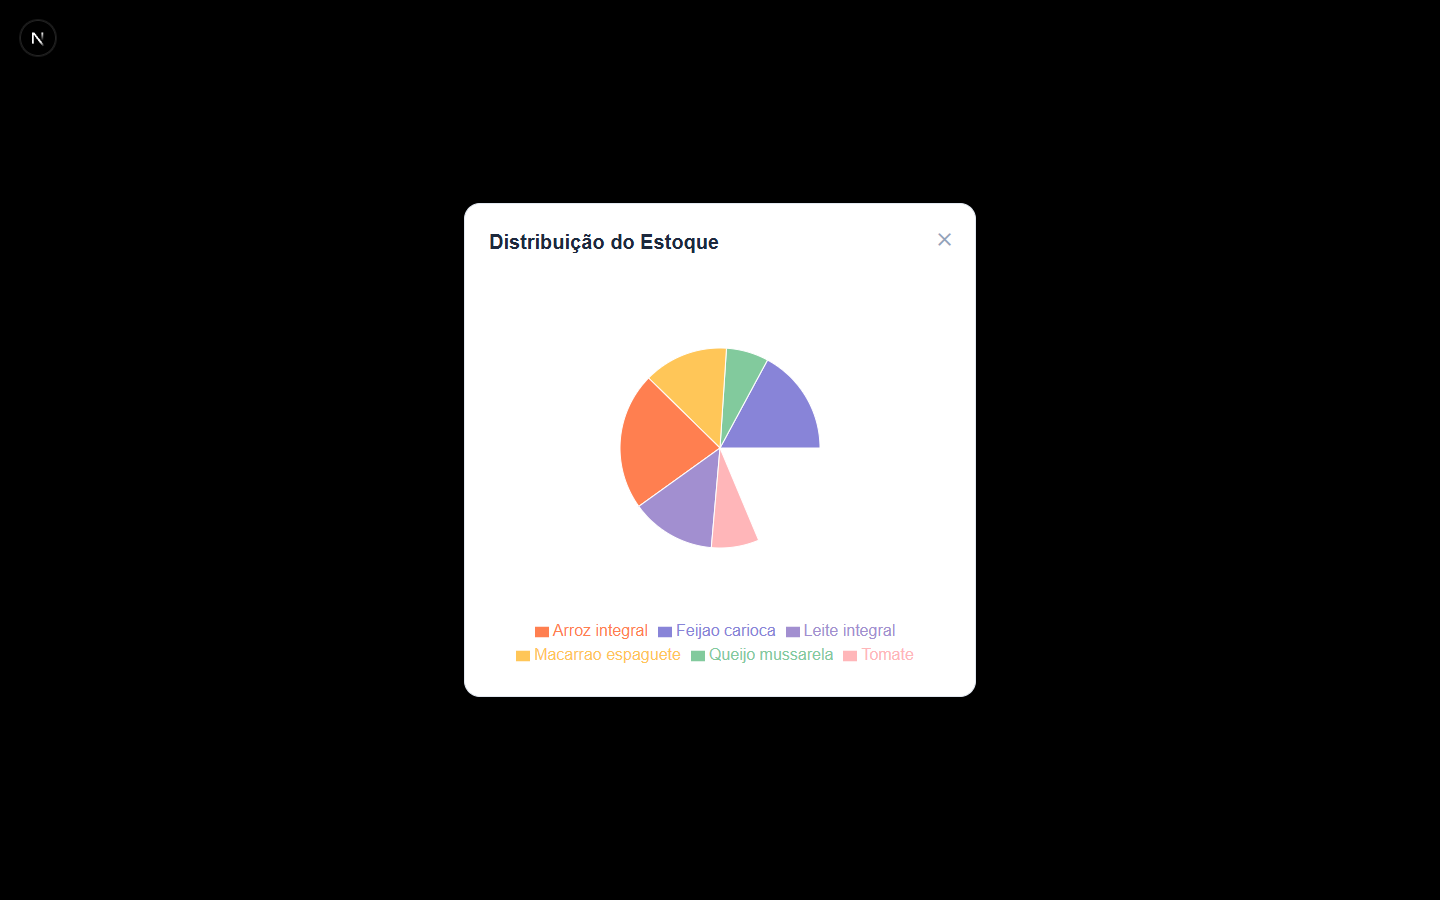
\includegraphics[width=\textwidth]{screenshots/07_dispensa_grafico_distribuicao.png}
    \caption{Grafico de distribuicao do estoque.}
\end{figure}

\begin{figure}[H]
    \centering
    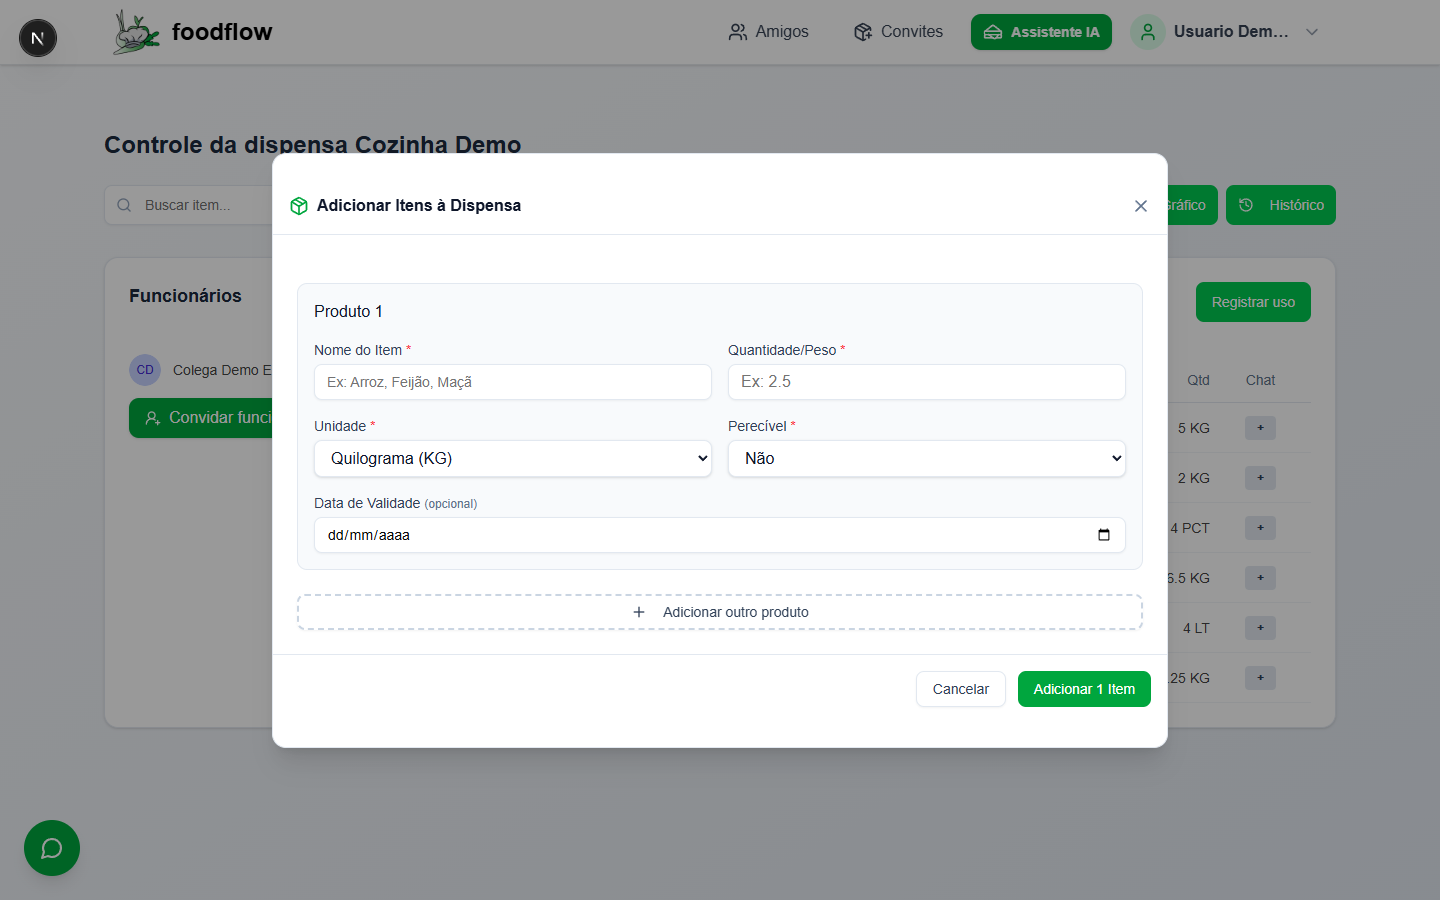
\includegraphics[width=\textwidth]{screenshots/08_modal_adicionar_item.png}
    \caption{Modal para adicionar itens a dispensa.}
\end{figure}

\begin{figure}[H]
    \centering
    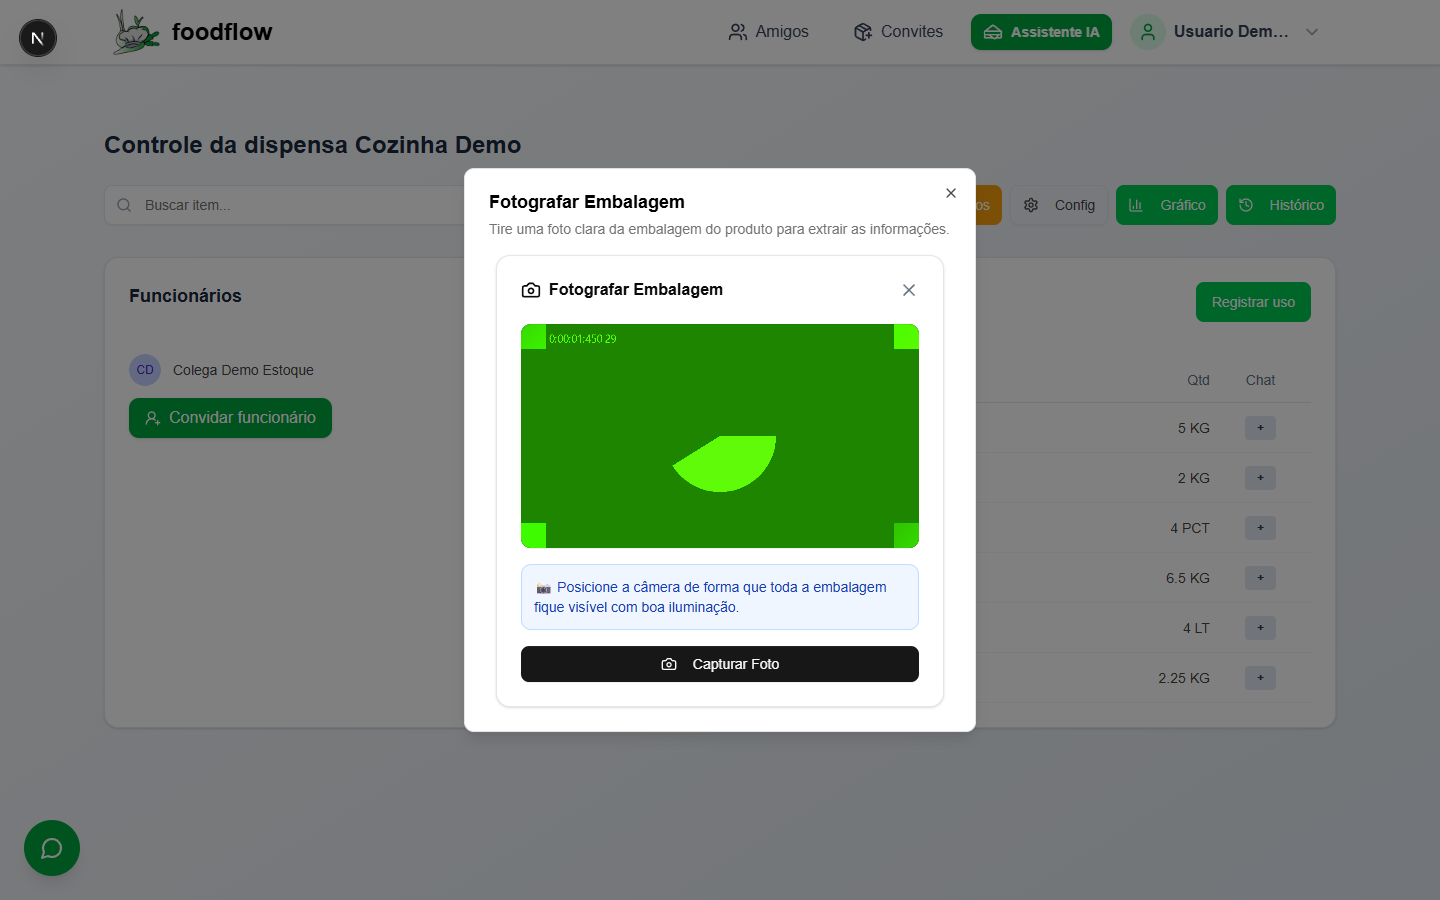
\includegraphics[width=\textwidth]{screenshots/09_modal_reconhecimento_embalagem.png}
    \caption{Fluxo de reconhecimento de embalagem por camera.}
\end{figure}

\begin{figure}[H]
    \centering
    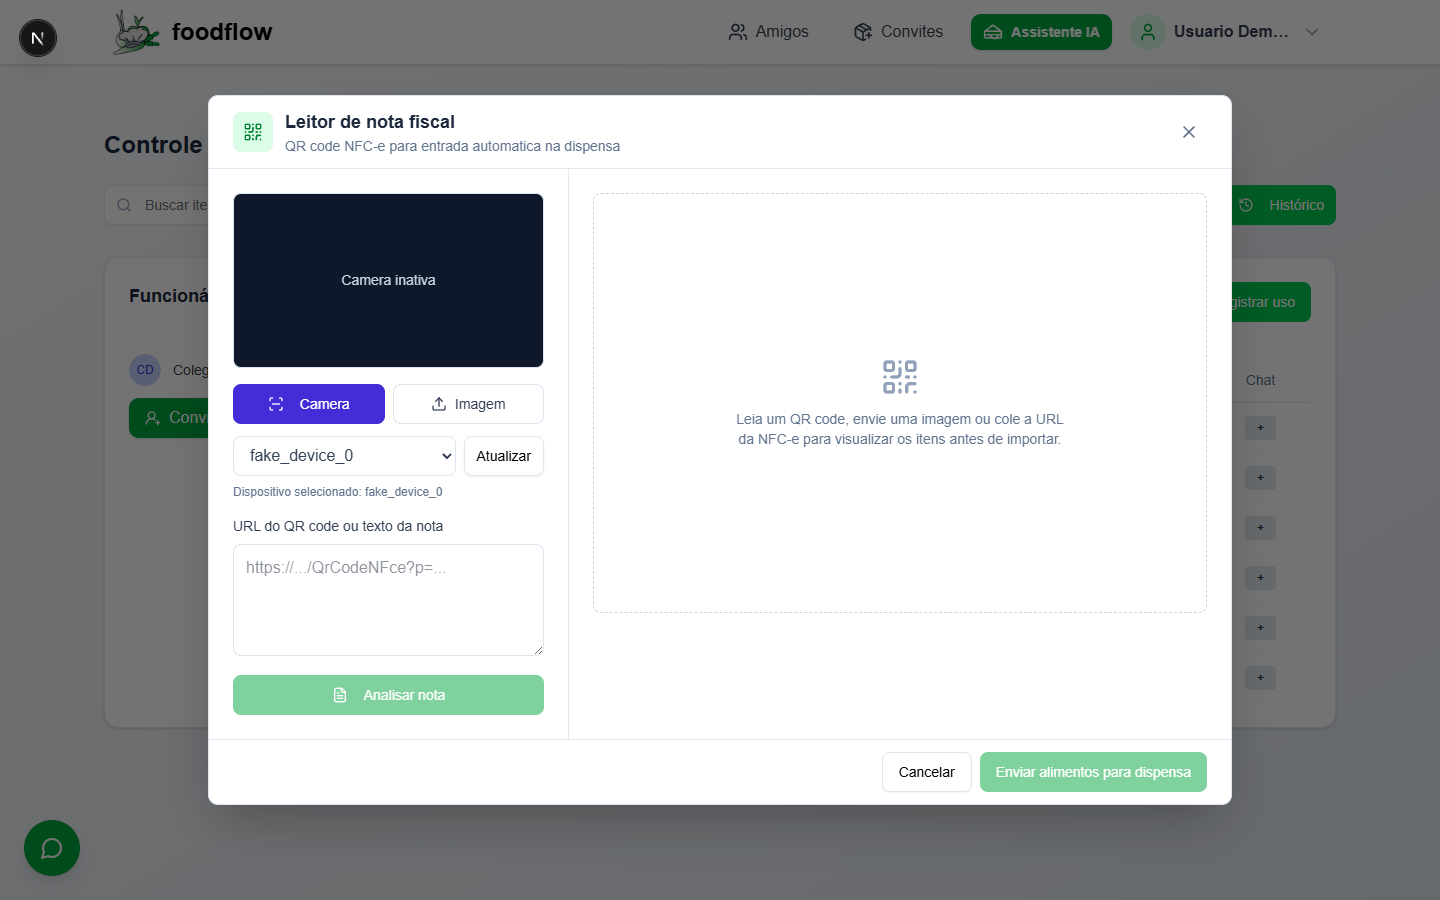
\includegraphics[width=\textwidth]{screenshots/10_modal_leitor_nota_fiscal.png}
    \caption{Leitor de nota fiscal NFC-e por QR code.}
\end{figure}

\begin{figure}[H]
    \centering
    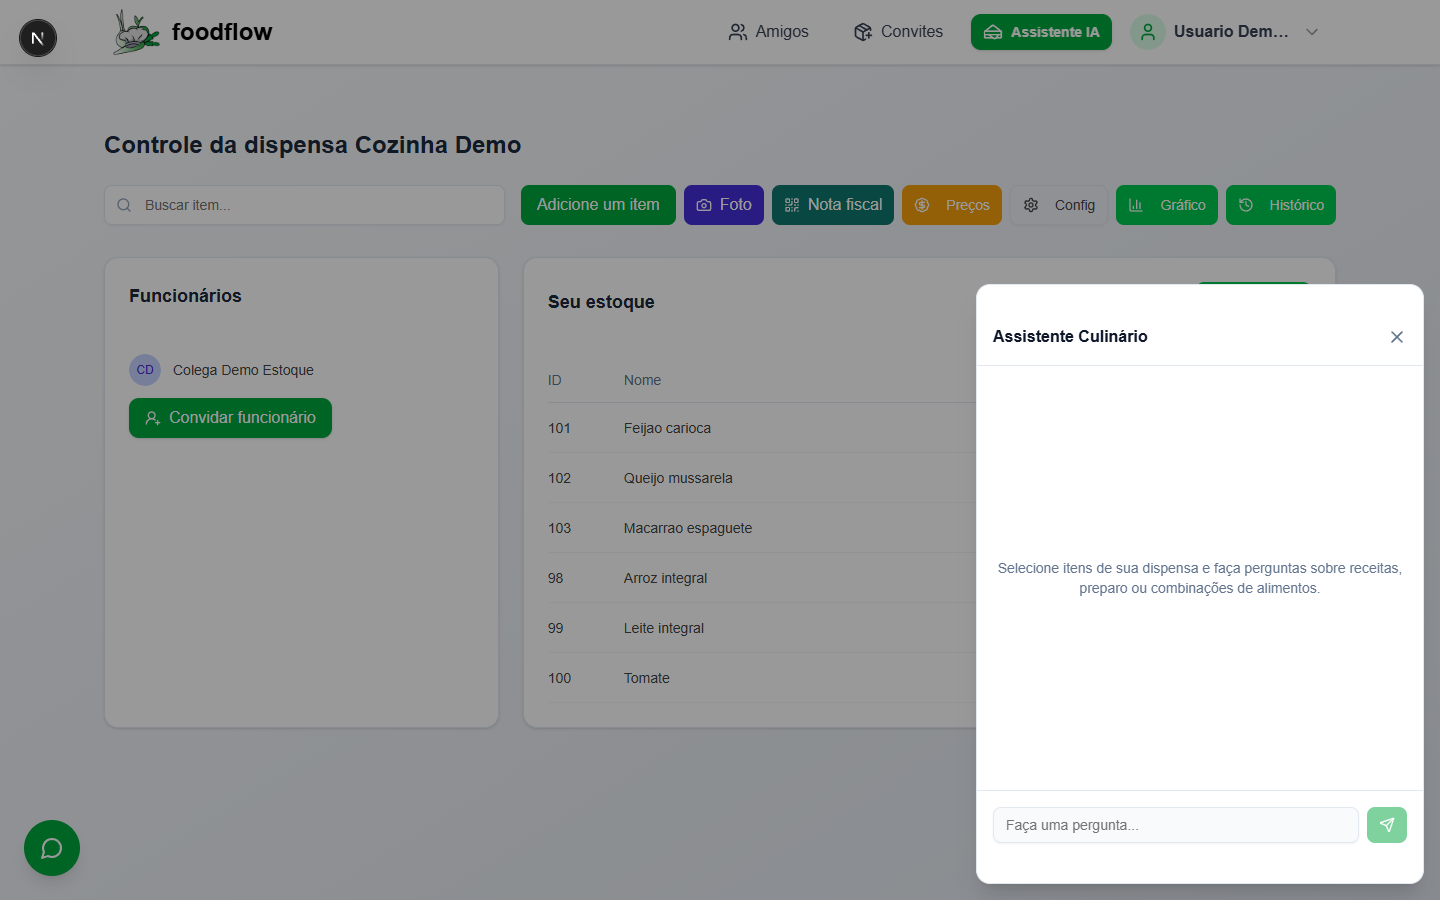
\includegraphics[width=\textwidth]{screenshots/11_assistente_culinario.png}
    \caption{Assistente culinario baseado em IA.}
\end{figure}

\begin{figure}[H]
    \centering
    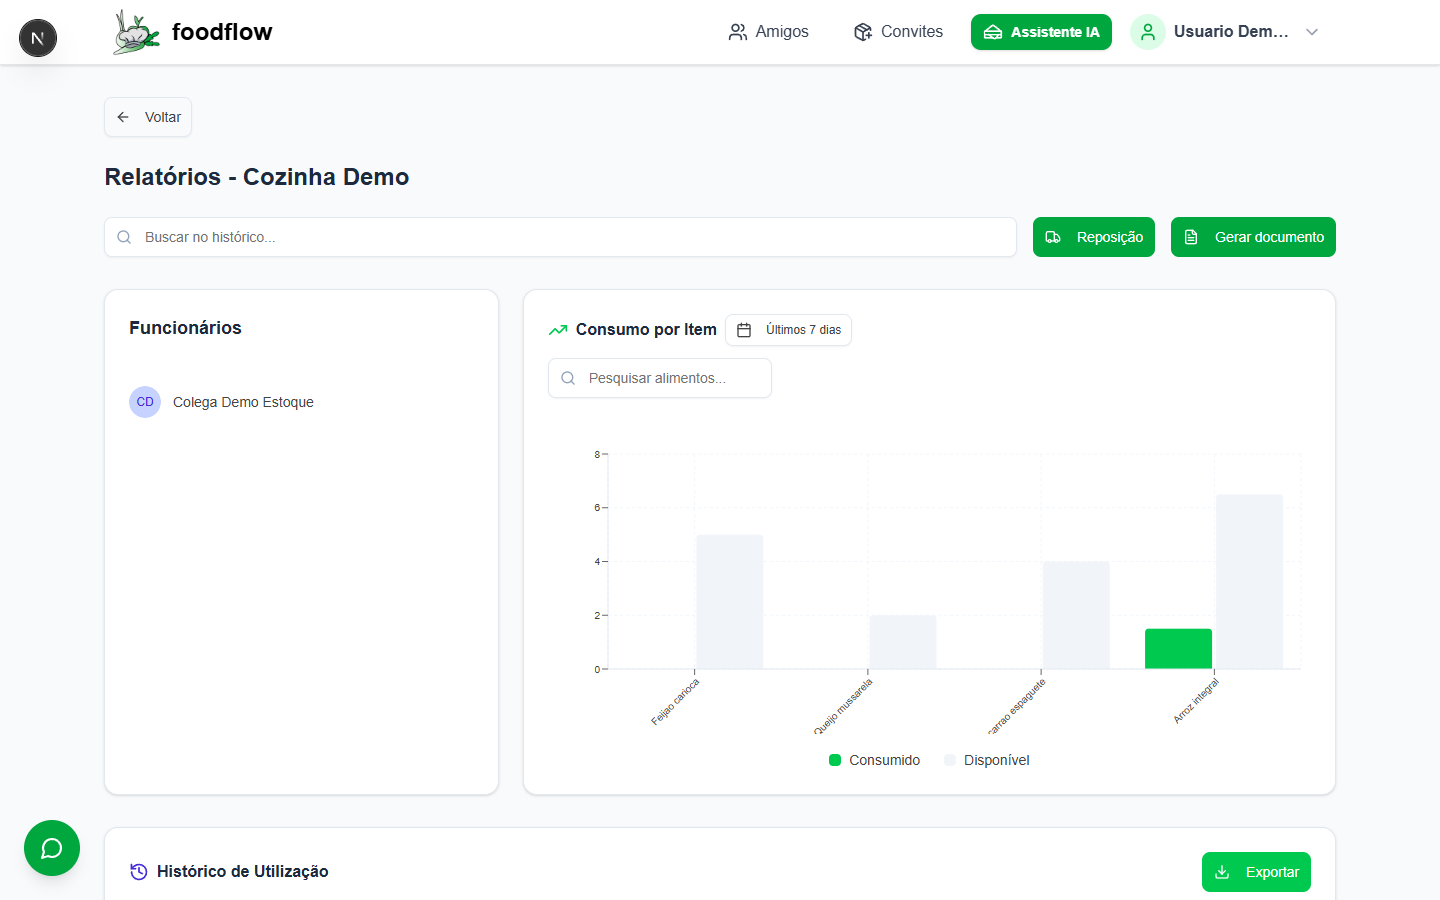
\includegraphics[width=\textwidth]{screenshots/12_relatorios_historico_consumo.png}
    \caption{Pagina de relatorios com historico e grafico de consumo.}
\end{figure}

\begin{figure}[H]
    \centering
    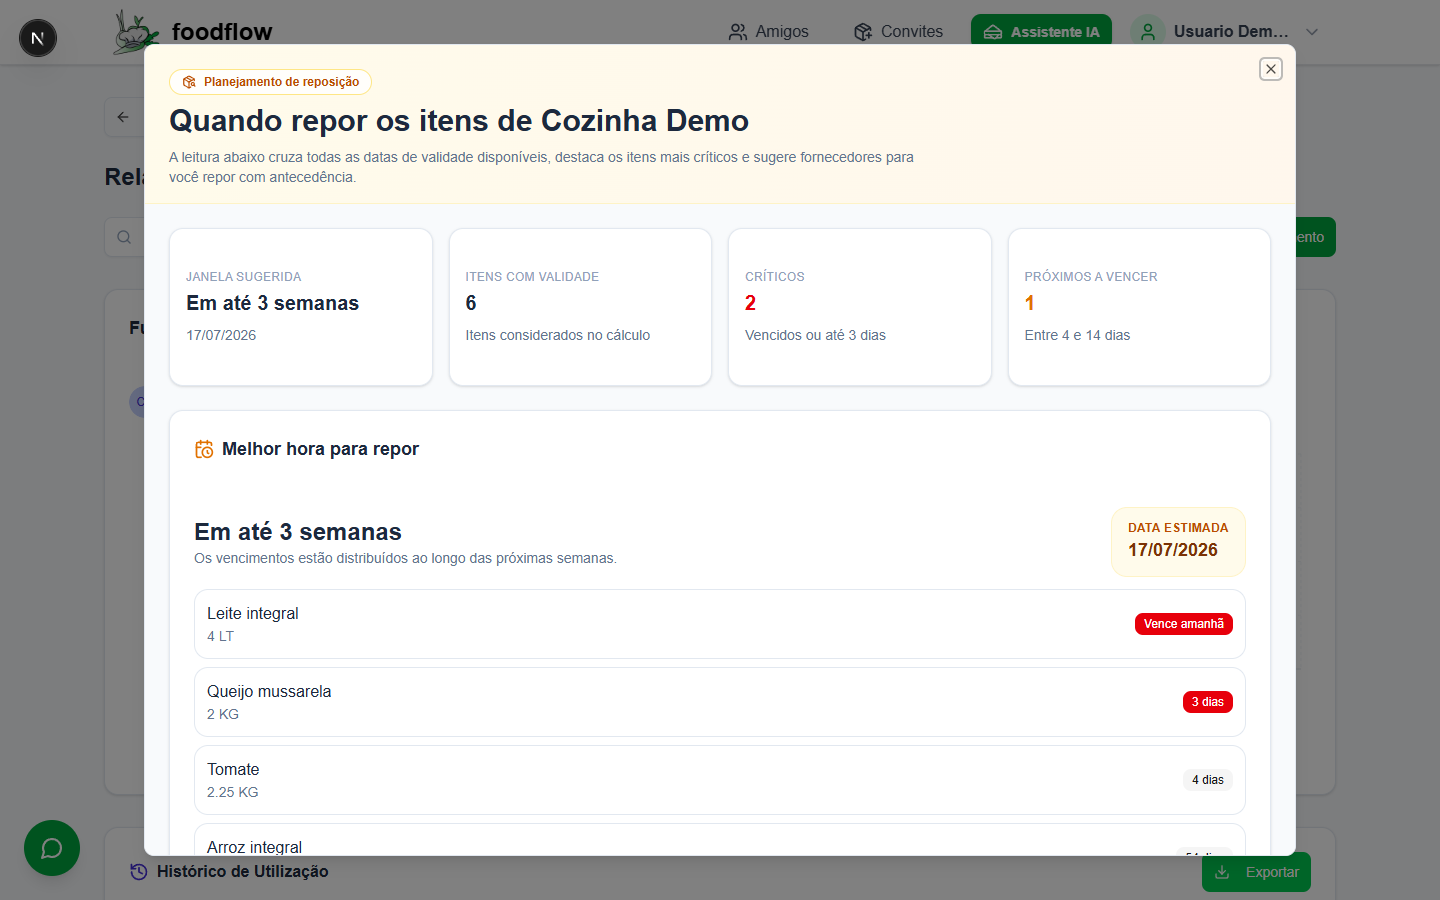
\includegraphics[width=\textwidth]{screenshots/13_modal_reposicao.png}
    \caption{Modal de planejamento de reposicao.}
\end{figure}

\begin{figure}[H]
    \centering
    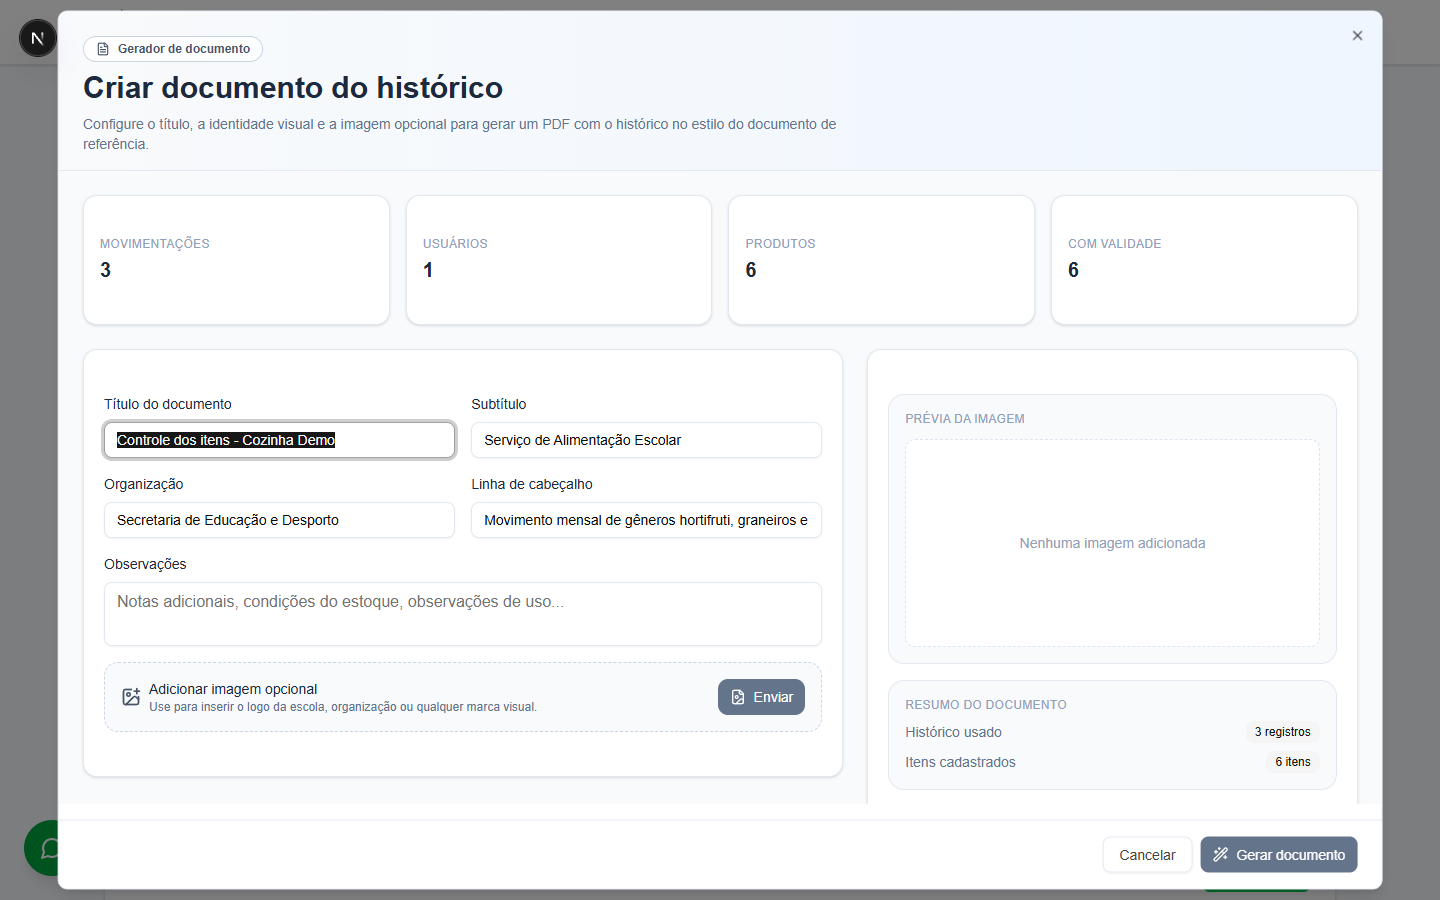
\includegraphics[width=\textwidth]{screenshots/14_modal_gerar_documento.png}
    \caption{Gerador de documento do historico.}
\end{figure}

\begin{figure}[H]
    \centering
    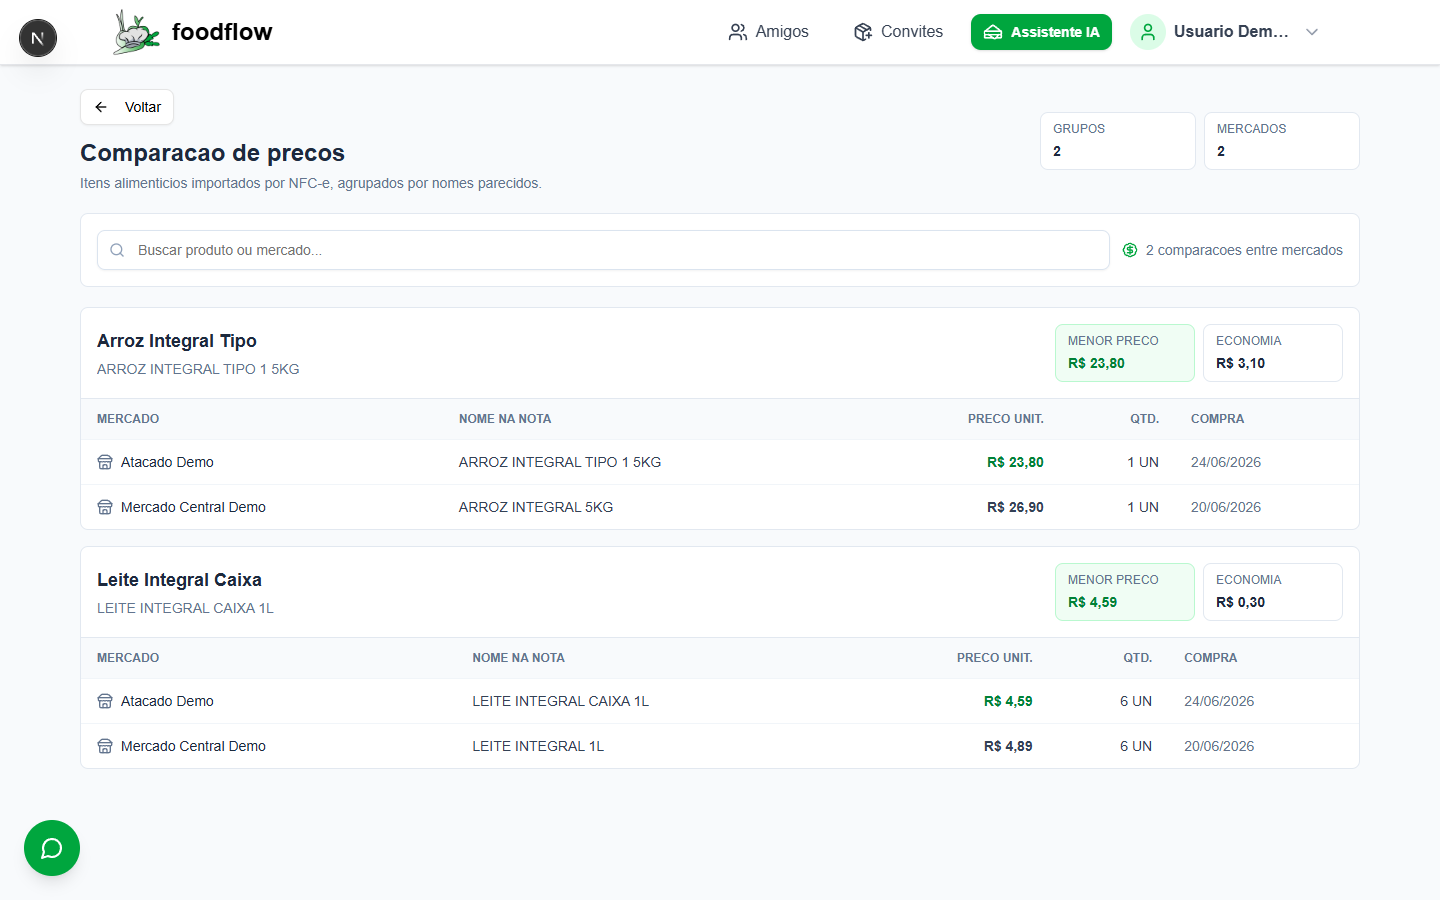
\includegraphics[width=\textwidth]{screenshots/15_comparacao_precos.png}
    \caption{Tela de comparacao de precos entre mercados.}
\end{figure}

\begin{figure}[H]
    \centering
    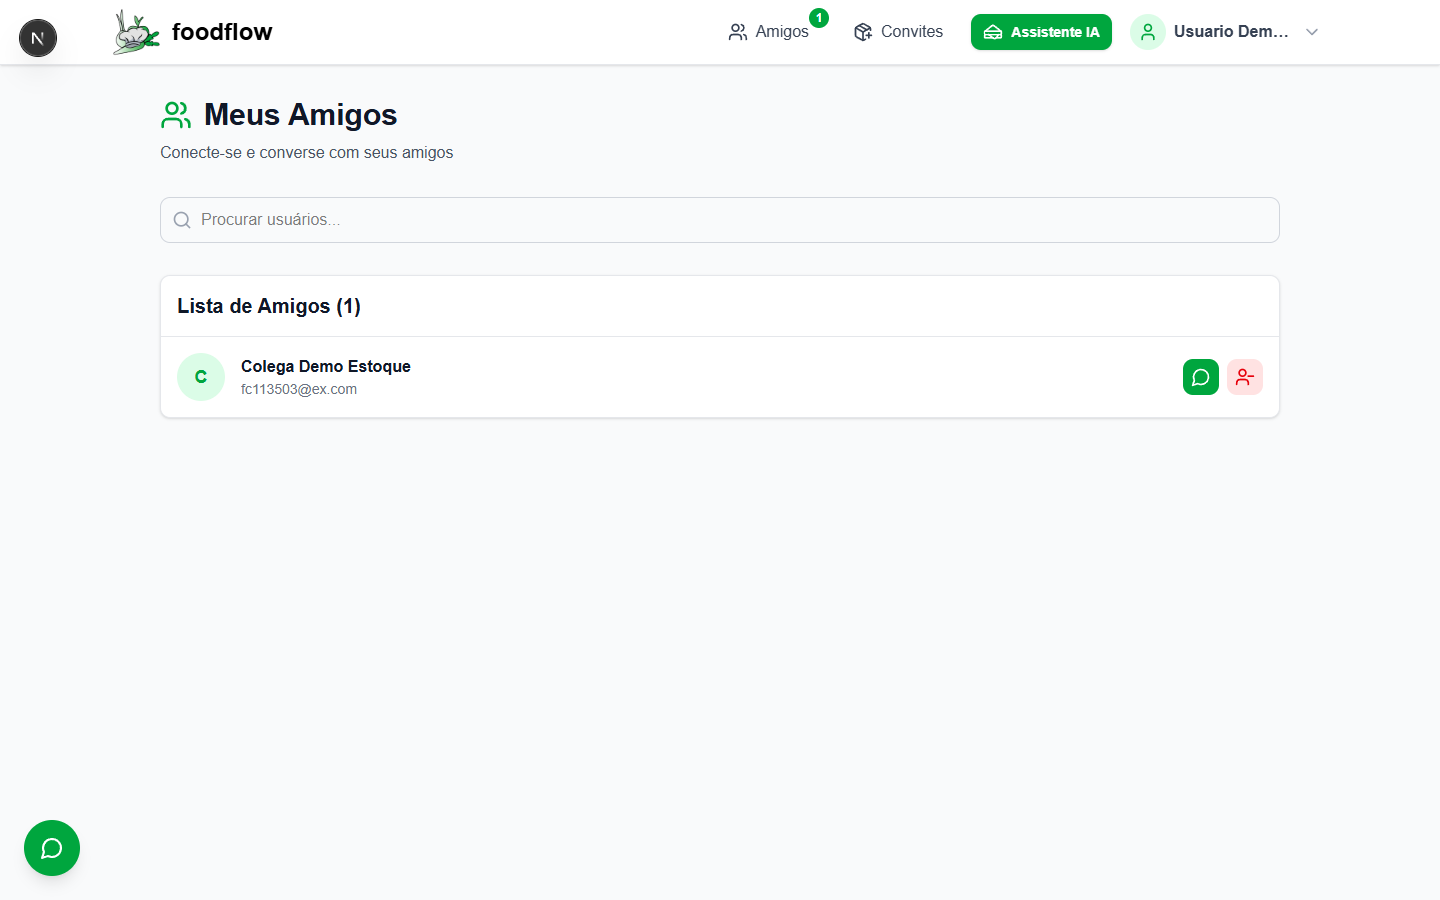
\includegraphics[width=\textwidth]{screenshots/16_amigos.png}
    \caption{Tela de amizades e lista de contatos.}
\end{figure}

\begin{figure}[H]
    \centering
    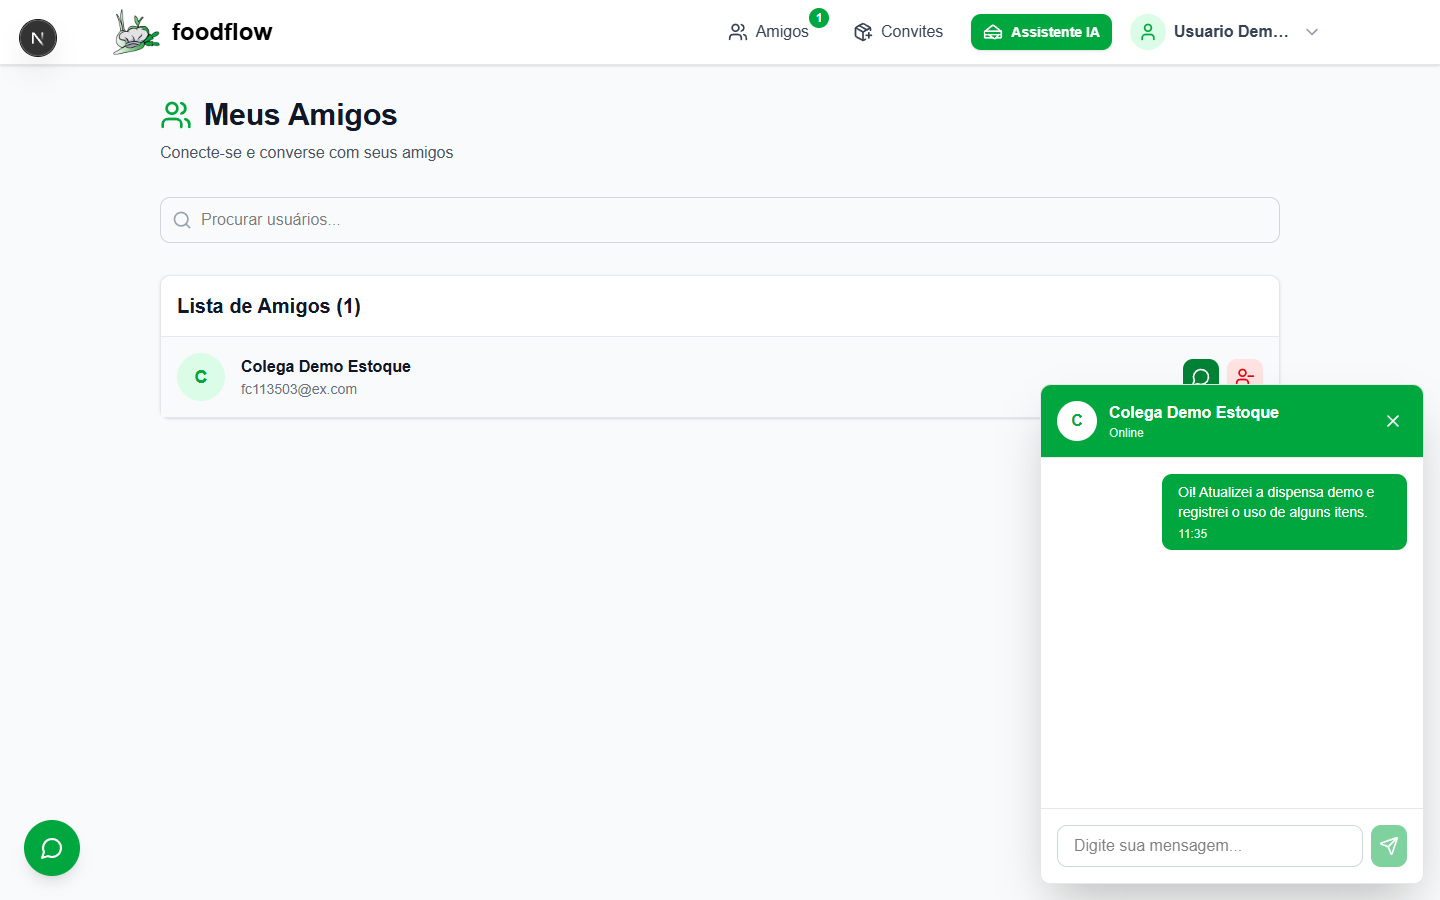
\includegraphics[width=\textwidth]{screenshots/17_chat_usuarios.png}
    \caption{Chat entre usuarios.}
\end{figure}
